%*****************************************
\chapter{Lambdapi}\label{ch:intro-lambdapi}
%*****************************************

\section{The \texorpdfstring{\lp}-Calculus modulo}

The \lp-calculus modulo rewriting (\lpm)  extends the Edinburgh Logical Framework (LF) \cite{lf} by allowing user-defined rewrite rules at both the term and type levels. 
In this framework, all terms and types are identified modulo the congruence relation generated by standard $\beta$-reduction together with the specified rewrite rules.
\lpm{}is implemented in the Lambdapi proof language \cite{lambdapi}, which is designed to facilitate proof exchange between systems.
Lambdapi, a successor of the Dedukti proof language \cite{Dedukti-ref, Dedukti-ref2}, differs primarily by offering an integrated proof tactic language. 
However, it can still import and export Dedukti theories to maintain compatibility.
Lambdapi/Dedukti was used to translate \cite{thire:tel-03224039} the Matita arithmetic library to several systems, including Coq and PVS, and to export \cite{blanqui:hal-04613926} the HOL Light standard library to Coq.

% \section{An assembly for proof assistant}

\begin{figure}[t]
    \centering
    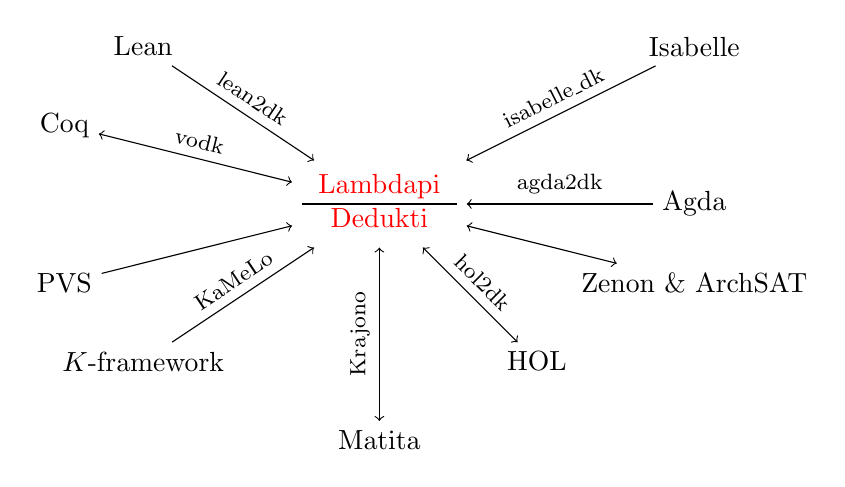
\begin{tikzpicture}
      \path (0,0) node (lp) {\begin{tabular}{c}
        \textcolor{red}{Lambdapi} \\
        \hline
        \textcolor{red}{Dedukti}
      \end{tabular}}
            (-4,1) node (coq) {Coq}
            (-3,2) node (lean) {Lean}
            % (0,2) node [draw, dashed, purple] (smt) {\color{purple}\textbf{SMT}}
            (4,2) node (isa) {Isabelle}
            (4,0) node (agda) {Agda}
            (-3,-2) node (k) {$\mathbb{K}$-framework}
            (0,-3) node (mat) {Matita}
            (2,-2) node (hol) {HOL}
            (-4,-1) node (pvs) {PVS}
            (4,-1) node (ze) {Zenon \& ArchSAT}
            ;
      % \draw[->,red, thick] (smt) -- (lp) node[midway,sloped,above]
      % {\footnotesize{Carcara}};
      \draw[->] (lean) -- (lp) node[midway,sloped,above] {\footnotesize{lean2dk}};
      \draw[->] (isa) -- (lp) node[midway,sloped,above] {\footnotesize{isabelle\_dk}};
      \draw[->] (agda) -- (lp) node[midway,sloped,above] {\footnotesize{agda2dk}};
      \draw[<->] (ze) -- (lp) node[midway,sloped,above] {};
      \draw[<->] (hol) -- (lp) node[midway,sloped,above] {\footnotesize{hol2dk}};
      \draw[<->] (mat) -- (lp) node[midway,sloped,above] {\footnotesize{Krajono}};
      \draw[->] (pvs) -- (lp);
      \draw[->] (k) -- (lp) node[midway,sloped,above] {\footnotesize{KaMeLo}};
      \draw[<->] (coq) -- (lp)  node[midway,sloped,above] {\footnotesize{vodk}};
    \end{tikzpicture}
    \caption{Lambdapi, an assembly language for proof systems.}
    \label{fig:interop}
\end{figure}

\section{Signature rules}

We start by defining the basic elements of the \lpm{} calculus and giving their syntax.
The terms of the \lp-Calculus Modulo are the same as in \lp-Calculus (LF).
The terms of \lpm{} are divided into three levels: objects (denoted by $M$ and $N$), types (denoted by $A$ and $B$), and kinds (denoted by $K$).
The syntax of \lpm{} is given by the following grammars:


\begin{flalign*}
&\text{Objects}  & M, N  &::= c \pipe x \pipe \lambda\,x : A, M \mathrel{|} M~N &\\
&\text{Types}   & A,B &::= a \pipe \Pi\,x:A, B \pipe A~M &\\
&\text{Kinds} & K & ::= \type \pipe \Pi\,x:A, K &\\
&\text{Terms} & t,u & ::= M \pipe A \pipe K \pipe \kind  &
\end{flalign*}

where $c$ is a constant and $x$ is a variable  (ranging over disjoint sets).
Dependent products  $\Pi\,x : A.\,B$ (respectively $\Pi\,x : A.\,K$) are simply written $A \rightarrow B$ when $x$ does not occur in $B$ (respectively $K$), $\lambda\,x : A.\,t$ is an abstraction, and  $t~v$ is an application.

\begin{definition}[Substitutions]
A substitution $\sigma$ is a function written \([ x_1 \leftarrow N_1, \dots, x_n \leftarrow N_n]\), from the set of variables to the set of terms with a finite domain.
We write $t\sigma$ the term $t$ where the variables are replaced by their image by $\sigma$.
\end{definition}

Contexts $\Gamma$ is a finite sequence of variable declarations $x:A$ introducing variables and their types.
A \emph{signature} \index{$\Sigma$} representing the \emph{global context} is a finite sequence of \emph{assumptions} $c : A$ (respectively $c:K$), indicating that constant $c$ is of type $C$ (respectively kind $K$), \emph{definitions} $c := A : M$, indicating that $c$ has the value $M$ and type $A$.
We write $\langle\rangle$ when context or signature are empty. Rewrite rules are pairs $M \re N$ (respectively $A \re B$), where the head symbol of $M$ (respectively $A$) are constants
and where free variables of $N$ (respectively $B$) occur in M (respectively $A$).

\begin{flalign*}
&\text{Contexts}  & \Gamma  &::= \langle\rangle \pipe \Gamma,x: A &\\
&\text{Signature} & \Sigma &::= \langle\rangle \pipe \Sigma, c: A \pipe \Sigma, a: K \pipe \Sigma, M \re N \pipe \Sigma,A \re B &
\end{flalign*}

The relation $\longrightarrow{\beta\Sigma}$ is generated by $\beta$-reduction and by the rewrite rules of $\Sigma$.
The relation $\longrightarrow_{\beta\Sigma}^*$ denotes the reflexive and transitive closure of $\longrightarrow_{\beta\Sigma}$, and the relation $\equiv_{\beta\Sigma}$ (called \emph{conversion}) the reflexive, symmetric, and transitive closure of $\longrightarrow_{\beta\Sigma}$. 

\section{Rewriting}

In the \lpm-Calculus we distinguish two kinds of rewriting.

\subsection{\texorpdfstring{$\beta$}{}-reduction}

The first kind of rewriting is $\beta$-reduction, which is defined as usual.

\begin{definition}[$\beta$-Reduction] The $\beta$-reduction relation $\longrightarrow_\beta$ is the smallest relation on terms containing
\( (\lambda x:A, u)v \longrightarrow_\beta u[x \leftarrow v] \) for any $A$, $u$ and $v$ and closed by subterm reduction.
\end{definition}

\begin{notation}
We write $\longrightarrow^*_\beta$ for the reflexive and transitive closure of $\longrightarrow_\beta$ and $\equiv_\beta$ for the congruence generated by $\longrightarrow_\beta$.
\end{notation}

\subsection{\texorpdfstring{$\Sigma$}{}-reduction}

The second kind of rewriting is $\Sigma-reduction$, the relation generated by the rewrite rules of a global context $\Sigma$.

\begin{definition}[$\Sigma$-Reduction]
Let $\Sigma$ be a global context. The  $\Sigma$-Reduction relation $\longrightarrow_\Sigma$ is the smallest relation on terms containing $u \longrightarrow_\Sigma v$
for each rule $u \re v \in \Sigma$ and closed by substitution and subterm reduction.
\end{definition}

\begin{notation}
We write $\longrightarrow_{\Sigma}$ for the reflexive and transitive closure of $\equivL$ for the congruence generated by $\longrightarrow^*_{\Sigma}$, $\longrightarrow^*_{\beta\Sigma}$,
for $\longrightarrow^*_{\beta} \cup \longrightarrow^*_{\Sigma}$, $\longrightarrow^*_{\Sigma}$ for the reflexive and transitive closure of $\longrightarrow^*_{\beta\Sigma}$ and $\equivL$
for the equivalence relation generated by $\longrightarrow_{\beta\Sigma}$.
\end{notation}

Lambdapi implements untyped rewriting because it will be inefficient to check the well-typedness of the substitution at each reduction step.
A Lambdapi typing judgment $\Gamma \vdash_\Sigma t : A$ asserts that term $t$ has type $A$ in the context $\Gamma$ and the signature $\Sigma$.

\begin{definition}[Linearity]
We also define the properties:
\begin{itemize}
\item A term is linear if no variable occurs twice in it;
\item A rewrite rule $M \re N$ is left-linear if $M$ is linear.
\end{itemize}
\end{definition}

\section{Typing system}
\label{sect:lambdapi}

We now give the typing rules of the \lpm{}-Calculus in \cref{fig:lp-typing-rules}. 

\begin{definition}[Well-Typed Term]
We say that a term $t$ has a type $A$ in global context $\Sigma$ and local context $\Gamma$ if the judgment $\Sigma,\Gamma \vdash t: A$ is
derivable by the inferences rules of \cref{fig:lp-typing-rules}. We say that a term is well-typed if such an $A$ exists.
\end{definition}

\begin{definition}[Well-Formed Local Context]
A local context $\Gamma$ is well-formed with respect to a global context $\Sigma$ if the judgment $\Sigma \vdash \Gamma$ is derivable by the inference rules of \cref{fig:lp-typing-rules}.
\end{definition}


\begin{figure}
  \[
    \begin{prooftree}
      \infer0[(Empty)]{ \vdash_\Sigma \langle\,\rangle  }
    \end{prooftree}
    \qquad
    \begin{prooftree}
      \hypo{ \vdash_\Sigma \Gamma }
      \hypo{ \Gamma \vdash_\Sigma A : s }
      \infer2[(Decl) $x \notin \Gamma$]{ \vdash_\Sigma \Gamma, x : A  }
    \end{prooftree}
  \]
  \medskip
  \begin{center}
    \begin{prooftree}
    \hypo{ \vdash_\Sigma \Gamma }
    \hypo{\Gamma \vdash_\Sigma A : s}
    \infer2[(Const)]{ \Gamma \vdash_\Sigma c : A }
    \end{prooftree}
  \end{center}
  \medskip
  \[
    \begin{prooftree}
      \hypo{ \vdash_\Sigma \Gamma } 
      \infer1[(Sort)]{ \Gamma \vdash_\Sigma \type : \kind }
    \end{prooftree}
    \qquad
    \begin{prooftree}
      \hypo{ \vdash_\Sigma \Gamma }
      \infer1[(Var) $x : A \in \Sigma$]{ \Gamma \vdash_\Sigma x : A }
    \end{prooftree}
  \]
  \medskip
  \begin{center}
    \begin{prooftree}
    \hypo{\Gamma, \vdash_\Sigma A : \type }
    \hypo{\Gamma, x: A \vdash_\Sigma B: s}
    \hypo{\Gamma, x : A \vdash_\Sigma t: B}
    \infer3[(Abs)]{ \Gamma \vdash_\Sigma \lambda x: A, t : \Pi x : A, B }
    \end{prooftree}
  \end{center}
  
  \begin{center}
    \begin{prooftree}
      \hypo{ \Gamma \vdash_\Sigma A : \type } 
      \hypo{ \Gamma, x : A \vdash_\Sigma B : s } 
      \infer2[(Prod)]{ \Gamma \vdash_\Sigma \Pi x : A, B : s }
    \end{prooftree}
    \quad
  \end{center}
  
  \medskip
  
  \begin{center}
    \begin{prooftree}
      \hypo{ \Gamma \vdash t : \Pi x : A, B }
      \hypo{ \Gamma \vdash  u : A }
      \infer2[(App)]{ \Gamma \vdash_\Sigma t~u : B[u \leftarrow x] }
    \end{prooftree} 
  \end{center}
  
  \medskip

  \begin{center}
  \begin{prooftree}
  \hypo{\Gamma, \vdash_\Sigma B: u}
  \hypo{\Gamma \vdash_\Sigma t: A}
  \hypo{A \textcolor{red}{\equiv_{\beta\Sigma}} B}
  \infer3[(Conv)]{ \Gamma \vdash_\Sigma t: B }
  \end{prooftree}
  \end{center}
  \caption{Typing rules of \lpm}
  \label{fig:lp-typing-rules}
  \end{figure}

\begin{remark}
The typing rules shown in \cref{fig:lp-typing-rules} are similar to those of  \lp{}-Calculus \cite[\S 2]{lf}, except for the additional rule (Conv) that identifies types modulo $\equivL$ instead of just modulo $\equiv_\beta$. 
\end{remark}

Besides the new conversion relation, the main difference between the \lp-Calculus and the \lpm-Calculus is the presence of the rewrite rules
in global contexts. We need to take this into account when typing global contexts. A key feature of any type system is the preservation of typing by reduction: the
subject reduction property.

\begin{definition}[Subject Reduction]
Let $\longrightarrow_r$ be a binary relation on terms.  
We say that a global context $\Sigma$ satisfies the \emph{subject reduction} property for $\longrightarrow_r$ if the following holds:  
for any well-formed local context $\Gamma$ with $\Sigma$, for any terms $t_1$ and $t_2$ such that $t_1 \longrightarrow_r t_2$, and for any term $T$,  
if $\Sigma, \Gamma \vdash t_1 : T$ then $\Sigma, \Gamma \vdash t_2 : T$.
\end{definition}

In the \lpm calculus, we can not allow adding arbitrary rewrite rules in the context if
we want to preserve properties such as subject reduction for relation $\longrightarrow_{\beta\Sigma}$.
Lambdapi requires user rules in $\longrightarrow_{\beta\Sigma}$ for the encoded theories to be \emph{confluent} (\cref{def:confluence-rew}),
even if it does not automatically check that this properties holds.

\begin{definition}[Confluent $\longrightarrow_{\beta\Sigma}$]\label{def:confluence-rew}
The relation $\longrightarrow_{\beta\Sigma}$ must be confluent, i.e., whenever $t \longrightarrow_{\beta\Sigma}^* v_1$ and $t \longrightarrow_{\beta\Sigma}^* v_2$, there exists a term $w$ such that $v_1 \longrightarrow_{\beta\Sigma}^* w$ and $v_2 \longrightarrow_{\beta\Sigma}^* w$, and it must preserve typing, i.e., 
whenever $\Gamma \vdash_\Sigma t\sigma: A$ with any substitution $\sigma$, and $t \longrightarrow_{\beta\Sigma} v$ then $\Gamma \vdash_\Sigma v\sigma: A$.
\end{definition}

In other words, confluence is a property of rewriting systems, describing that if terms in such a system can be rewritten in more than one way, to yield the same result. 

\begin{remark}
External tools such as CSI \cite{CSI} can be used to check the confluence of a set of rewriting rules with a Signature.
Lambdapi can export its rules and the signature $\Sigma$ in a format accepted by CSI. 
\end{remark}

One approach to prove the confluence property that we will now describe is to check that the critical pairs (\cref{def:critical-pair}) of the rewrites rules in $\Sigma$ are joinable.

\begin{definition}[Position and Subterm]
Let $t$ be a term. We denotes $Post(t)$ the set of position in $t$ that is a sequences of integers and the subterm $t_{| p}$ of $t$
at position $p \in Post(t)$ are defined inductively as follows:
\begin{itemize}
  \item if $t$ is a variable, then $Post(t) = \{ \epsilon \}$ and $t_{| \epsilon} = t$;
  \item if $t = f~t_1 \dots t_n$, then \( Post(t) = \{ \epsilon \} \cup \{1.q \pipe q \in Post(t_1)\} \cup \dots \cup \{n.q \pipe q \in Post(n_1)\} \),
    \( t_{| \epsilon} = t \text{ and } t_{| i.q} = t_{| i.q} \).
  
\end{itemize}
\end{definition}

\begin{definition}[Critical pair]\label{def:critical-pair}
Let $l_i \re r_i$ (for $i = 1, 2$) be two rewrite rules. Suppose that they do not share any variable (variables can be renamed if needed).
If there exists $p \in Post(l_1)$ such that $l_{1 | p}$ is not a variable and $\sigma$ is a most general unifier of $l_{1 | p}, l_2$ then
we have the following reduction $\l_1sigma \re (l_1\sigma)[l_2\sigma]_p$. We say that the pair $((l_1\sigma)[l_2\sigma]_p, r_1\sigma)$ is a
critical pair and that the two rewrite rules overlop.
\end{definition}

\begin{theorem}[Critical Pair Theorem]\label{thm:cp}
The set of rewrites rules $R$ over the signature $\Sigma$ (and its set of variables $\cal{V}$) have  is locally confluent if and only if its critical pairs are joinable.
\end{theorem}


\begin{lemma}[Newman’s Lemma]\label{lem:newman}
Let $(A, \re)$ be an abstract reduction system. If $\re$ is \emph{terminating} (i.e., there is no infinite sequence 
$x_0 \re x_1 \re x_2 \re \cdots$) and \emph{locally confluent} (i.e., for all $s,u,v \in A$, if $s \re u$ and $s \re v$ then there exists 
$c \in A$ such that $u \re^{*} c$ and $v \re^{*} c$), then it is confluent (i.e., for all $s,u,v \in A$, if $s \re^{*} u$ and 
$s \re^{*} v$ then there exists $w \in A$ such that $u \re^{*} w$ and $v \re^{*} w$).
\end{lemma}

\begin{remark}
Similar than confluence, Lambdapi does not check itself that a set of rules terminates.
However, external tools such as Approve \cite{aprove} can be used to check the termination of a set of rewriting rules with a Signature.
Lambdapi can export its definitions and Signature into a format accepted by the tool Approve.
\end{remark}

Combining \cref{thm:cp} with Newman's (\cref{lem:newman}) we get the following result:

\begin{corollary}
The set of rewrites rules $R$ over the signature $\Sigma$ is confluent if and only if its critical pairs are joinable.
\end{corollary}

\section{Prelude}
\label{sec:prelude-lp}

The Lambdapi standard library comes with the following definitions that we will reuse and that we contributed to enrich.

\begin{definition}[Prelude Encoding]
\label{def:defuniv}
The signature $\Sigma$ of our encoding contains the following definitions and rewrite rules that we use to encode Alethe proofs:
\begin{align*}
&\set\index{\set}: \type & &\prop\index{\prop}: \type \\
&\index{\el{}} \el{}: \set \rightarrow \type  & &\index{\prf}\prf{} : \prop \rightarrow \type \\
&\mathop{\leadsto}\index{$\leadsto$}: \set \rightarrow \set \rightarrow \set \quad \text{(infix)} & &o: \set \\
&\el\,(x \leadsto y) \hookrightarrow \el\,x \rightarrow \el\,y & &\el\,o\index{o}  \hookrightarrow \prop
\end{align*}
\end{definition}

The notions of term, proposition, and proof are not primitive in \lpm.
We first define a notion analogous to the predicate logic notion of term, to express the objects the theory speaks about, such as the natural number.
The constants \set{} and \prop{} in \cref{def:defuniv} are type universes ``à la Tarski'' \cite[\S Universes]{intuitype} in \lpm.
The type \set{} represents the universe of \textit{small types}, i.e.\ a subclass of types for which we can define equality.
Since elements of type \set{} are not types themselves,
we also introduce a function $\el: \set \rightarrow \type$ that embeds the terms of type \set{} into terms of type \type.

Jus as \lpm{} does not contain a primitive notion for expressing the objects of the theory, it does not contain a primitive notion of proposition.
The constant \prop{} represents the universe of propositions. Predicate symbols are represented as constants of type $\set{} \ra \dots \ra \prop$ .
Similar to \set{}, elements of type \prop{} are not types themselves; they are mapped to types by the function $\prf{}: \prop \rightarrow \type$.
Drawing an analogy with the Curry-de-Brujin-Howard isomorphism \cite{curryhoward}, this function embeds propositions into types by mapping each proposition $A$ to the type $\prf\,A$, which represents its proofs.
However, the analogy is only partial in two important ways. First, the propositions themselves are not the types of their proofs: if $t$ is a proof of $A$, then it does not have the type $A$,
but the type $\prf\,A$. Second, the embedding is not surjective—meaning not all types correspond to proofs. For instance, neither \set{} nor \prop{} are themselves types of proofs.

Consequently, a \emph{step} in an Alethe proof trace is represented as an inhabitants of type $\prf{}\,p$, for a suitable proposition $p$.

\section{Constructive connectives, quantifiers and classical facts}
\label{ssec:encoding-prop}

In our framework, we adopt the standard set of logical operators and axioms from intuitionistic logic.

\begin{definition}[Constructive connectives, quantifiers]
\begin{align}
& \top : \prop \\
& \bot : \prop \\
& \land : \prop \ra \prop \ra \prop \qquad \text{(written infix)} \\
& \lor : \prop \ra \prop \ra \prop \qquad \text{(written infix)} \\
& \Rightarrow : \prop \ra \prop \ra \prop \qquad \text{(written infix)} \\
&  \prf\,(a \Rightarrow\,b) \re \prf\, a \ra \prf\,\,b \label{eq:imp}\\
& \neg a \is a \Rightarrow \bot \\
% & \mathop{\mathrm{xor}}~a~b \is (\neg a \land b) \lor (a \land \neg b) \\
& \forall : \Pi {[a: \set]}, (\el\, a \ra \prop) \ra \prop \label{eq:forall}\\
& \prf{}(\forall\,p) \re \Pi\, x, \prf{(p~x)}\\
& \exists : \Pi\, {[a: \set]}, (\el\, a \ra \prop) \ra \prop \\
& {=} : \Pi [a : \set], \el\, a \ra \el\, a \ra \prop \qquad \text{(written infix)}
\end{align}
\end{definition}

According to the Curry-de Bruijn-Howard correspondence, a proof of $A \Rightarrow B$ should have the type $\prf\,(A \Rightarrow B)$.
However, such a proof actually has type $\prf\,A \ra \prf\,B$. This means that the types $\prf\,(A \Rightarrow B)$ and $\prf\,A \ra \prf\,B$ must be identified.
To achieve this, we introduce the rewriting rule \cref{eq:imp}, allowing $\prf\,(A \Rightarrow B)$ to be rewritten as $\prf\,A \ra \prf\,B$.

We cannot assign the type $\Pi : \type, (X \ra \prop) \ra \prop$ to the universal quantifier, because in \lpm{} there is no mechanism for quantifying over variables of type \type.
Instead, we assign the type $\Pi\,x:\set{},(\el\,x \ra \prop) \ra \prop$ to the generic universal quantifier $(\forall)$ \cref{eq:forall}.
Furthermore, the previously defined term $o: Set$, together with the rewrite rule $\el\,o\index{o}  \hookrightarrow \prop$
, enables quantification over propositions, rendering the universal quantifier impredicative.

\begin{example}[quantification over $\prop$ with $o$]
The eliminator for bottom can be formalized as:
\[ \bot_e : \prf\,(\bot \Rightarrow \forall (p: \el\,o), p) \]
\end{example}

Equality (=) over small types is parameterized over types $\el\,a$ for the type parameter $a : \set{}$.

\subsection{Inductive data structure}

To illustrate how inductive types are expressed in Lambdapi, we present below some data structure.
While this example is primarily intended to demonstrate the syntax and capabilities of the system, the same structure will later be employed in our encoding in \cref{ch:encoding}.
Lambdapi extends the \lpm-Calculus Modulo by providing partial support for inductive types.
An inductive type is declared by specifying its name, followed by a list of constructors, each describing one possible way of building an element of the type.
The general form is:

\begin{align*}
&TypeName : \type\\
&|~constructor1 : \dots : TypeName \\
&|~constructor2 : \dots : TypeName\\
&\dots
\end{align*}

This support is described as partial because Lambdapi currently does not enforce the positivity constraint on inductive definitions.
From any inductive type declaration, Lambdapi automatically derives the corresponding induction principle along with its associated inference rules.


\begin{definition}[Product type]\label{def-product}
The product type, which pairs together values from two types, is constructed as follows:
\begin{align*}
&\textbf{Non dependent product type:} \\
&\quad \times : \text{Set} \to \text{Set} \to \text{Set} \quad \textit{(written infix)} \\
&\textbf{Pairing symbol:} \\
&(\mathbin{‚}) [a~b] : \el a \ra \el b \ra \el (a \times b)\\[1em]
&\textbf{Projections (written postfix):}  \\
&\quad {}_1 : \el\, (a \times b) \ra \el\, a \quad \text{with rewrite rule } (x \mathbin{‚} \_)_1 \re x \\
&\quad {}_2 : \el\, (a \times b) \ra \el\, b \quad \text{with rewrite rule } (\_ \mathbin{‚} y)_2 \re y
\end{align*}
\end{definition}

\begin{definition}[List]\label{def:list}
The structure of a list is specified through the following inductive type definition:
\begin{align*}
&[a: \set]~ \bb{L}: \type \\
&|~\Box : \bb{L}~a \\
&|~\mathrel{::}~: \el  a \ra \bb{L}~a \ra \bb{L}~a \quad \text{(written infix)} \\[1em]
& \kw{list}~: \set \ra \set \\
&  \el~\kw{list}~a \re \bb{L}~a
\end{align*}
\end{definition}

The pairing constructor is denoted by $(‚)$ (a comma-like symbol), which takes two terms $x : \el\,a$ and $y : \el\, b$ and produces a term $x \mathbin{‚} y : \el (a \times b)$.
Two projection symbols ${\_}_1$ and ${\_}_2$ extract the first and second components of a pair, respectively.

\begin{definition}[Dependent pair]\label{dep-pair-def}
The type $\Sigma~p$ parameterized by a predicate $p$ on a type $\el\,a$, represents a dependent pair consisting of an element $x : \el\,a$ and a proof that $p~x$ holds.

\begin{align*}
&\Sigma : \forall a : \set{}, (\el{}~a \ra \prop): \type \\
&|~exist : \Pi (a : \set{}), \prf (p~x) \ra \Sigma~p \\
&\\
& Sigma~[a: \set{}]: (\el{}~a \ra \prop) \ra \set{} \\
& \el{}~Sigma~p \re \Sigma~p \\
&\\
& \textcolor{red}{s_1}~[a: \set{}] [p:(\el{}~a \ra \prop)] (e: \Sigma~a~p): \el{}~a \\
& (exist~x~\_)~\textcolor{red}{s_1} \re x\\
& s_2~[a: \set{}] [p:(\el{}~a \ra \prop)] (e: \Sigma~a~p): \prf{}(p~(e~\textcolor{red}{s_1})) \\
& (exist~x~p)~s_2 \re p\\
\end{align*}
The projections from this dependent pair are defined through the symbols $s_1$ and $s_2$, corresponding respectively to the first and second components of the pair.
The rewrite rule for $s_1$ extracts the value $x$ from a term of the form $\kw{exist}~x~\_$, while the rule for $s_2$ retrieves the proof that $(p~x)$ holds.
\end{definition}

\begin{definition}[Dependent vector]\label{def:dependent-vector}
since both the size of the collection and the type of its elements influence how the predicate is computed.
Let \( a : \set \), we define the constant \( \mathop{\mathrm{Vec}}~a~n \) inductively for \( n : \N \) as:
\begin{align*}
&[a: \set] \mathop{\mathrm{Vec}}: \N \ra \type \\
&|~\Box_\bb{V} : \mathop{\mathrm{Vec}}\,a\, 0 \\
&|~\mathbin{::}_\bb{V}\,[n:\N]: \el\,a \ra \mathop{\mathrm{Vec}}\,a\,n \ra  \mathop{\mathrm{Vec}}\,a\,(n +1) \quad (\text{infix})\\
&\mathop{\mathrm{vector}}: \set \ra \N \ra \set \\
&\el~(\mathop{\mathrm{vector}}~a~(n: \N)) \re \mathop{\mathrm{Vec}}~a~n \\[1em]
& \kw{distinct}~[a: Set] [n: \N] : \kw{Vec}~a~n \ra \prop
\end{align*}
\end{definition}